\documentclass[3p,authoryear]{elsarticle}
\journal{Annals of Nuclear Energy}

%%%%%%%%%%%%%%%%%%%%%%%%%%%%%%%%%%%%%%%%%%%%%%%%%%%%%%%%%%%%%%%%%%%%%%%%%%%%%%%%
\usepackage[charter]{mathdesign} % Type-1 Latin Modern modern
\usepackage[T1]{fontenc}         % Use T1 encoding instead of OT1
\usepackage[utf8]{inputenc}      % Use UTF8 input encoding
\usepackage{microtype}           % Improve typography
\usepackage{booktabs}            % Publication quality tables
\usepackage{amsmath}
\usepackage{float}
\usepackage{algorithm}
\usepackage{algorithmicx}
\usepackage{algpseudocode}
\usepackage[exponent-product=\cdot]{siunitx}

\usepackage{color}
\definecolor{aneblue}{RGB}{0,128,173}
\usepackage[colorlinks,breaklinks]{hyperref}
\AtBeginDocument{
  \hypersetup{linkcolor=aneblue, citecolor=aneblue, urlcolor=aneblue}
}

% Captions for figures and tables
\usepackage[labelfont=bf]{caption}
\captionsetup[figure]{labelsep=period, name=Fig.}
\captionsetup[table]{labelsep=newline}

% Set correct abbreviations
\def\equationautorefname{Eq.}
\def\figureautorefname{Fig.}

\DeclareMathOperator\erfc{erfc}

% Fix transparency in figures
% \pdfpageattr {/Group << /S /Transparency /I true /CS /DeviceRGB>>}

%%%%%%%%%%%%%%%%%%%%%%%%%%%%%%%%%%%%%%%%%%%%%%%%%%%%%%%%%%%%%%%%%%%%%%%%%%%%%%%%
\begin{document}

\title{Comparison of algorithms for Doppler broadening pointwise tabulated cross
  sections}

\author[bmpc]{Paul K. Romano\corref{cor1}}
\ead{paul.romano@unnpp.gov}
\cortext[cor1]{Corresponding author. Tel.: +1 518 395 4010.}

\author[bmpc]{Timothy H. Trumbull}
\ead{timothy.trumbull@unnpp.gov}

\address[bmpc]{Bechtel Marine Propulsion Corporation -- Knolls Atomic Power
  Laboratory \\ P.O. Box 1072, Schenectady, NY 12301, United States}

\begin{abstract}
  In this paper, three algorithms for Doppler broadening pointwise tabulated
  cross sections are compared on the basis of speed and accuracy. The use of a
  Gauss-Legendre quadrature for numerical integration on subintervals of the
  convolution integral for which the cross section is smooth was found to reduce
  run time by 48\% compared to the exact method used in NJOY and other cross
  section processing codes. However, a comparable decrease in run time was also
  achieved simply by using a more efficient implementation of the $\erfc$
  function. The use of a Gauss-Hermite quadrature for performing the convolution
  integral resulted in an order of magnitude decrease in run time for
  broadening. The accuracy of the Gauss-Hermite quadrature was also studied, and
  it was found that quadrature orders greater than 15 reach an asymptotic level
  of error. Lastly, an on-the-fly implementation of Doppler broadening in OpenMC
  using a Gauss-Hermite quadrature resulted in at least a factor of 15 increase
  in run time relative to a simulation without Doppler broadening for the BEAVRS
  benchmark problem, underscoring the need for advanced methods for on-the-fly
  temperature treatment for Monte Carlo codes.
\end{abstract}

\begin{keyword}
  Doppler broadening, algorithms, Gauss-Legendre quadrature, Gauss-Hermite
  quadrature
\end{keyword}

\maketitle

%%%%%%%%%%%%%%%%%%%%%%%%%%%%%%%%%%%%%%%%%%%%%%%%%%%%%%%%%%%%%%%%%%%%%%%%%%%%%%%%
\section{Introduction}

For use in Monte Carlo particle transport codes, cross sections are typically
represented as a series of pointwise tabulated functions of energy that are
linearly interpolated between tabulated values. The tabulations themselves are
generated with a processing code such as NJOY and are constructed such that
linear interpolation between tabulated points gives values that are accurate to
a specified error level. A cross section library is typically stored only for a
single temperature.

Historically, the most common approach to handling the dependence of cross
sections on temperature is to Doppler broaden cross sections at 0 K to the
desired temperature before the simulation is run. For problems containing
materials at multiple temperatures, cross sections would need to be generated
for each temperature present. Alternatively, interpolation between bracketing
temperatures could be used, an idea explored thoroughly by
\citet{nse-trumbull-2006}.

More recently, several methods have been proposed for Doppler broadening cross
sections \textit{on-the-fly}, i.e. during the neutron transport simulation
rather than as a pre-processing step. The first of these on-the-fly methods was
proposed by \citet{nse-yesilyurt-2012} where the dependence of a cross section
on temperature is expanded as a series of polynomials. By storing the 0 K cross
sections and a series of polynomial expansion coefficients, the cross section
can be calculated at any temperature with high accuracy. This approach would
require approximately 6 GB of memory to store the 0 K cross sections and
polynomial expansion coefficients for all nuclides in ENDF/B-VII.1
\citep{snamc-brown-2013}.

Another method for accounting for multiple temperatures using only 0 K data is
the target motion sampling method \citep{nse-viitanen-2012}. This approach is
quite different in the sense that an effective Doppler broadened cross section
is never calculated. Rather, a rejection sampling technique is used on the
neutron path length to account for the fact that the total cross section is a
distributed quantity.

Lastly, \citet{ane-forget-2014} demonstrated that Doppler broadening could be
performed on-the-fly if cross sections are stored in a multipole representation
rather than as pointwise tabulated functions. This method offers the prospect of
drastically reducing the memory required for cross sections while being able to
handle problems with many temperatures, but it is still under active
development.

The purpose of the present work is to thoroughly compare existing methods for
Doppler broadening pointwise tabulated cross sections. These algorithms are
typically used in cross section processing codes such as NJOY
\citep{lanl-macfarlane-2012}, AMPX \citep{tans-dunn-2002}, and Fudge
\citep{nds-mattoon-2012}, although some have been proposed as potential
on-the-fly algorithms as well.

\subsection{Doppler-broadening Equation}

The effects of thermal motion of the target nuclei can be taken into account by
calculating an effective cross section defined by averaging the reaction rate in
such a way that it is preserved:
\begin{equation}
  \label{eq:reaction-rate}
  v \sigma(v,T) = \int d\mathbf{V} \; |\mathbf{v} - \mathbf{V}|
  \sigma_0(|\mathbf{v} - \mathbf{V}|) P(\mathbf{V},T)
\end{equation}
where $\mathbf{v}$ is the velocity of the neutron, $\mathbf{V}$ is the velocity
of the target nuclide, $\sigma_0(v)$ is the \SI{0}{\kelvin} cross section at
incoming speed $v$, $\sigma(v,T)$ is the effective cross section at incoming
speed $v$ and temperature $T$, and $P(\mathbf{V},T)$ is the velocity
distribution of the target nuclei at temperature $T$. By assuming that
$P(\mathbf{V},T)$ is a Maxwellian distribution, it can be shown that
\autoref{eq:reaction-rate} reduces to the well-known Doppler broadening equation
\citep{ornl-wigner-1944}
\begin{equation}
  \sigma (v,T) = \frac{1}{v^2} \left ( \frac{\beta}{\pi} \right )^{1/2}
  \int_0^{\infty} dv_r \; v_r^2 \sigma(v_r,T_0) \left [ e^{-\beta (v - v_r)^2} -
    e^{-\beta (v + v_r)^2} \right ]
\end{equation}
where $v_r = |\mathbf{v} - \mathbf{V}|$ is the speed of the neutron relative to
the target, $T_0$ is some temperature less than $T$, and $\beta = \frac{M}{2k(T
  - T_0)}$ where $M$ is the target mass and $k$ is Boltzmann's constant. It is
convenient to define the variables
\begin{eqnarray}
  y^2 = \beta v^2 \\
  x^2 = \beta v_r^2
\end{eqnarray}
and to make a change of variables from $v_r$ and $v$ to $x$ and $y$. Doing so
yields
\begin{equation}
  \label{eq:broaden-xy}
  \sigma (y,T) = \frac{1}{y^2\sqrt{\pi}} \int_0^{\infty} dx \; x^2 \sigma(x,T_0)
  \left [ e^{-(x - y)^2} - e^{-(x + y)^2} \right ].
\end{equation}
By defining
\begin{equation}
  \label{eq:sigma-star}
  \sigma^* (y,T) = \frac{1}{y^2\sqrt{\pi}} \int_0^{\infty} dx \; x^2
  \sigma(x,T_0) e^{-(x - y)^2}
\end{equation}
we can then write \autoref{eq:broaden-xy} as two separate pieces
\begin{equation}
  \sigma(y,T) = \sigma^*(y,T) - \sigma^*(-y,T).
\end{equation}
The problem of Doppler broadening a cross section is thus reduced to performing
the integral in \autoref{eq:sigma-star}. The challenging aspect of this integral
is that the dependence of the cross section on $x$ can not be expressed in
closed form. As mentioned earlier, the cross section is usually represented as a
series of tabulated points and is linearly interpolated between points.

It is customary to restrict the range of integration in
\autoref{eq:sigma-star}. Since the term $e^{-(x-y)^2}$ becomes small for $|x-y|$
large, the range of integration is typically taken to be $-4 \le x - y <
4$. \citet{nse-cullen-1976} have shown that the error introduced by truncating
the range of integration is negligibly small.

%%%%%%%%%%%%%%%%%%%%%%%%%%%%%%%%%%%%%%%%%%%%%%%%%%%%%%%%%%%%%%%%%%%%%%%%%%%%%%%%
\section{Algorithms}

In this work, we will compare three different algorithms for Doppler broadening
pointwise cross sections. The first is a method known as SIGMA1, named after the
code in which it was first implemented \citep{nse-cullen-1976}. This method, or
a slight variant of it, is used in most major cross section processing codes,
including NJOY and AMPX. We will refer to this method as the
\textit{piecewise-linear exact integration} method to distinguish it from the
other methods, which are not exact.

A variation on the exact integration method was proposed by
\citet{physor-li-2012} aimed at achieving a faster, but potentially less
accurate, algorithm. While the authors called this method FDB (Fast Doppler
Broadening), we will instead refer to it as the \textit{Gauss-Legendre} method
as it relies on a Gauss-Legendre quadrature over small, fixed subintervals.

Lastly, a different approach was proposed by \citet{nd-dean-2010} wherein
\autoref{eq:sigma-star} is numerically integrated using a Gauss-Hermite
quadrature rather than being evaluated by subdividing it into intervals. This
method, the \textit{Gauss-Hermite} method, can dramatically reduce the number of
floating point operations needed, but, like the Gauss-Legendre method, this
comes at the expense of accuracy.

Before presenting results comparing the methods, we first begin by describing
how each of these methods solves the integral in \autoref{eq:sigma-star}.

\subsection{Piecewise-linear Exact Integration}

If the cross section is a piecewise linear function, the integral in
\autoref{eq:sigma-star} can be exactly integrated over each interval for which
the cross section is smooth. Over each smooth subinterval, we can express the
cross section as
\begin{equation}
  \label{eq:piecewise-linear}
  \sigma(x) = \sigma_i + s_i (x^2 - x_i^2), \quad \forall x \in [x_i, x_{i+1})
\end{equation}
where $s_i = (\sigma_{i+1} - \sigma_i)/(x_{i+1}^2 - x_i^2)$. Note that we have
not written the dependence on temperature for simplicity. To make use of
\autoref{eq:piecewise-linear}, we first express the integral in
\autoref{eq:sigma-star} as a sum of integrals over each smooth subinterval:
\begin{equation}
  \label{eq:sigma-star-interval}
  \sigma^* (y,T) = \frac{1}{y^2\sqrt{\pi}} \sum_i \int_{x_i}^{x_{i+1}} dx \;
  x^2 \sigma(x, T_0) e^{-(x-y)^2}.
\end{equation}
Then, by substituting \autoref{eq:piecewise-linear} into
\autoref{eq:sigma-star-interval} and simplifying, one can show that
\citep{lanl-macfarlane-2012}
\begin{align}
  \label{eq:sigma1}
  \sigma^* (y,T) &= \frac{1}{y^2\sqrt{\pi}} \sum_i \left[ \left( \sigma_i - s_i
    x_i^2 \right) \left( \frac{1}{y} H_2 - \frac{2}{y} H_1 + H_0 \right) +
    \right. \nonumber \\ & \qquad\qquad\qquad \left. s_i \left( \frac{1}{y^2}
    H_4 - \frac{4}{y} H_3 + 6 H_2 - 4y H_1 + y^2 H_0 \right) \right]
\end{align}
where $i$ is an index for each interval $[x_i, x_{i+1})$ and $H_n$ is shorthand
  for $H_n(x_i - y, x_{i+1} - y)$. The function $H_n$ is defined as $H_n(a,b) =
  F_n(a) - F_n(b)$ where
\begin{align}
  F_0(a) &= \frac{1}{2} \erfc (a) \\
  F_1(a) &= \frac{1}{2\sqrt{\pi}} e^{-a^2} \\
  F_2(a) &= \frac{1}{4} \erfc(a) + \frac{1}{2\sqrt{\pi}} ae^{-a^2} \\
  F_3(a) &= \frac{1}{2\sqrt{\pi}} e^{-a^2} \left ( 1 + a^2 \right ) \\
  F_4(a) &= \frac{3}{8} \erfc (a) + \frac{1}{2\sqrt{\pi}} e^{-a^2} \left (
  \frac{3}{2} a + a^3 \right )
\end{align}
Since $F_2$, $F_3$, and $F_4$ can be defined in terms of $F_0$ and $F_1$, this
means that for each smooth subinterval, i.e., at each point on the energy grid
within the range of integration, one evaluation of the exponential function and
one evaluation of the complementary error function is required. This can be
quite expensive computationally, but it is exact given a piecewise-linear cross
section.

\subsection{Gauss-Legendre Quadrature}

Noting that evaluations of the complementary error function can be expensive,
\citet{physor-li-2012} chose to perform the integration in
\autoref{eq:sigma-star-interval} by using a two-point Gauss-Legendre quadrature
over each interval where $\sigma$ is smooth. The Gauss-Legendre quadrature is
defined as
\begin{equation}
  \int_{-1}^1 dx \; f(x) \approx \sum_{k=1}^N w_k f(r_k)
\end{equation}
where $r_k$ are the roots of the Legendre polynomials and $w_k$ are the weights
of the quadrature which can be determined as
\begin{equation}
  w_k = \frac{2}{\left ( 1 - r_k^2 \right ) \left [ P'_n (r_k) \right ]^2}
\end{equation}
where $P'_n(r_k)$ is the derivative of the $n$th order Legendre polynomial
evaluated at $r_k$.  For a two-point quadrature, the roots of the second-order
Legendre polynomial are simply $r = \pm \sqrt{1/3}$ and the weights are
unity. Since the limits of integration on the integral in
\autoref{eq:sigma-star-interval} are not $-1$ to $1$, it is necessary to
transform the normal Gauss-Legendre quadrature to one appropriate for using over
any finite interval $[a,b]$:
\begin{equation}
  \label{eq:gauss-legendre-ab}
  \int_{a}^b dx \; f(x) \approx \frac{b-a}{2} \sum_{k=1}^N w_k f\left(
  \frac{b-a}{2} r_k + \frac{a+b}{2} \right).
\end{equation}
Thus, using \autoref{eq:gauss-legendre-ab} and \autoref{eq:sigma-star-interval},
we obtain\footnote{In \citet{physor-li-2012}, the transformation factor of
  $(x_{i+1} - x_i)/2$ outside the sums was missing from the final expression.}
\begin{equation}
  \label{eq:gauss-legendre}
  \sigma^* (y,T) = \frac{1}{y^2\sqrt{\pi}} \sum_i \frac{x_{i+1} - x_i}{2}
  \sum_{k=1}^N w_k f \left ( \frac{x_{i+1} - x_i}{2} r_k + \frac{x_i +
    x_{i+1}}{2} \right )
\end{equation}
where $f(x) = x^2 \sigma(x) e^{-(x-y)^2}$.

Comparing \autoref{eq:gauss-legendre} with \autoref{eq:sigma1}, we see that the
obvious benefit of the Gauss-Legendre quadrature method is the avoidance of
complementary error function evaluations. In densely packed energy grids where
$x_{i+1} - x_i$ is quite small, a two-point Gauss-Legendre quadrature provides a
highly accurate approximation to the analytical expression. However,
\citet{physor-li-2012} noted that for cases where $x_{i+1} - x_i > 1$, the
accuracy of the quadrature may degrade. Thus, they chose to revert to the exact
integration method in such cases.

\subsection{Gauss-Hermite Quadrature}

A different approach taken by \citet{nd-dean-2010} is to use a Gauss-Hermite
quadrature to evaluate the integral in \autoref{eq:sigma-star} rather than
subdividing the integral into intervals over which the cross section is
smooth. This enables the integral to be performed with potentially much fewer
cross section lookups---only as many as the quadrature requires.

To cast \autoref{eq:sigma-star} into a form suitable for using a Gauss-Hermite
quadrature requires a change of variables from $x$ to $z = x - y$, leading to
\begin{equation}
  \label{eq:sigma-star-z}
  \sigma^* (y,T) = \frac{1}{y^2\sqrt{\pi}} \int_{-y}^{\infty} dz \; (z + y)^2
  \sigma(z,T_0) e^{-z^2}.
\end{equation}
Recall that a Gauss-Hermite quadrature is defined as
\begin{equation}
  \int_{-\infty}^{\infty} dz \; e^{-z^2} f(z) \approx \sum_{k=1}^N w_k f(z_k)
\end{equation}
where $z_k$ are the roots of the Hermite polynomial $H_n(z)$ and $w_k$ are the
weights of the quadrature which can be determined as
\begin{equation}
  w_k = \frac{2^{n-1} n! \sqrt{\pi}}{n^2 \left [ H_{n-1} (z_k) \right ]^2}.
\end{equation}
For the integral in \autoref{eq:sigma-star-z}, the function to be evaluated is
$f(z) = (z+y)^2 \sigma(z,T_0)$.

One issue with using a Gauss-Hermite quadrature for \autoref{eq:sigma-star-z} is
that the lower limit of integration is not $-\infty$. Thus, the quadrature will
only work well when $y$ is large. As mentioned earlier, the range of integration
is typically restricted to $-4 \le z < 4$, implying that the Gauss-Hermite
quadrature will work for $y > 4$ or, in terms of energy, $E > 16kT/A$.

No mention was made by \citet{nd-dean-2010} about how to handle broadening when
$y < 4$. That being said, they did observe errors up to 2\% at low energies
using the Gauss-Hermite quadrature that may have resulted from an additional
approximation. Our approach in this paper will be to only use Gauss-Hermite
quadrature for $y > 4$ and revert to the exact integration method for $y < 4$.

%%%%%%%%%%%%%%%%%%%%%%%%%%%%%%%%%%%%%%%%%%%%%%%%%%%%%%%%%%%%%%%%%%%%%%%%%%%%%%%%
\section{Results}

A code called NADA (NAtive Doppler Application) was written to test the
different Doppler broadening algorithms. NADA operates on cross section
libraries in the HDF5 \texttt{ND\_LIBRARY} format, which is used for the MC21
Monte Carlo particle transport code \citep{snamc-griesheimer-2013}. NADA has the
capability to read cross section data at a base temperature from an
\texttt{ND\_LIBRARY}, Doppler broaden it (in parallel via MPI), and then write
out the broadened data to a new \texttt{ND\_LIBRARY}. For the present purposes,
no parallelism was used for Doppler broadening since we are primarily interested
in the serial execution time.

\subsection{Piecewise-Linear Integration Methods}

The piecewise-linear exact integration method and the Gauss-Legendre quadrature
method both perform Doppler broadening by evaluating the integral in
\autoref{eq:sigma-star-interval}. In the former method, the integral is
evaluated symbolically and found to be a combination of polynomials, $\exp$
functions, and $\erfc$ functions. The $\erfc$ function is the most difficult to
evaluate and accounts for a significant fraction of the run-time in this method.

At the time NJOY/BROADR was written, Fortran did not include the $\erfc$
function as an intrinsic function. Thus, NJOY uses an implementation of $\erfc$
from the SLATEC Common Mathematical Library which in turn is based on the MP
Multiple-Precision Package \citep{acm-brent-1978}. The Fortran 2008 standard now
includes $\erfc$ as an intrinsic function for real arguments, and support for
this intrinsic is available in most modern compilers (e.g., Intel, GNU, and PGI
all support this intrinsic). In most cases, the compiler implementation for a
common mathematical function like $\erfc$ is already highly optimized and will
likely outperform a hand-written implementation.

A cross section library was created using the NDEX nuclear data processing code
with each of following nuclides at \SI{293.6}{\kelvin}: $^{238}$U, $^{235}$U,
$^{233}$U, $^{232}$Th, $^{239}$Pu, $^{240}$Pu, $^{16}$O, and $^{56}$Fe. The
aforementioned nuclides were then broadened to \SI{600}{\kelvin},
\SI{900}{\kelvin}, and \SI{1200}{\kelvin} using NADA with three separate Doppler
broadening implementations:
\begin{enumerate}
\item Piecewise-linear exact integration using the $\erfc$ function from NJOY,
\item Piecewise-linear exact integration using the Fortran 2008 $\erfc$
  intrinsic function, and
\item Piecewise-linear integration using a Gauss-Legendre quadrature over each
  interval $[x_k, x_{k+1}]$.
\end{enumerate}
While NADA is in general capable of performing adaptive energy grid refinement
and grid thinning, these features were turned off for this
comparison. \autoref{tab:piecewise-integration} shows a comparison of timing
results for the three Doppler broadening implementations on an Intel Xeon
E5-2670 processor.
\begin{table}[H]
  \centering
  \caption{Observed wall-clock time to Doppler broaden eight selected nuclides
    to three temperatures.}
  \label{tab:piecewise-integration}
  \begin{tabular}{lc}
    \toprule
    Method & Time (s) \\
    \midrule
    Exact integration (NJOY \texttt{erfc}) & 32.5 \\
    Exact integration (Fortran 2008 \texttt{erfc}) & 21.2 \\
    Gauss-Legendre quadrature & 16.8 \\
    \bottomrule
  \end{tabular}
\end{table}

The results in \autoref{tab:piecewise-integration} are consistent with
previously reported results. \citet{physor-li-2012} found that using a
Gauss-Legendre quadrature for performing the integration over each interval
gained them a speedup of 2--3 over using the BROADR module of NJOY. However,
they did not mention whether or not adaptive energy grid refinement and grid
thinning was applied in their code. While the Gauss-Legendre quadrature method
does reduce the run time by 48\% compared to the exact integration method using
NJOY's $\erfc$ function, simply changing from NJOY's $\erfc$ implementation to
the intrinsic $\erfc$ function results in a 35\% reduction in run time.

\subsection{Gauss-Hermite Quadrature}

The paper by \citet{nd-dean-2010} left a number of open questions regarding the
use of the Gauss-Hermite quadrature for Doppler broadening. While the argument
that the Gauss-Hermite quadrature method should significantly outperform the
exact integration method was compelling based on theoretical considerations
alone, no comparisons of run time between the two methods was actually given. In
addition, the performance will depend on the order of the quadrature, but
\citet{nd-dean-2010} did not mention what order quadrature they had
used. Furthermore, only one example of the accuracy of the method was given
which showed unexplained oscillatory behavior of the error at low energy.

To better understand the speed and accuracy of the Gauss-Hermite quadrature
method, we studied the performance of a version of NADA that implemented this
method. The basis for comparison was the same eight nuclide test suite used to
compare the exact integration method to the Gauss-Legendre method. As before,
each nuclide was broadened from \SI{293.6}{\kelvin} to three temperatures. The
test suite was run iteratively starting with a 5 point quadrature and going up
to a 30 point quadrature. \autoref{fig:runtime} shows the observed wall-clock
time to run the test suite as a function of the order of the quadrature. As
expected, an increasing quadrature order increases the wall-clock time, but even
for larger quadratures the run time is vastly lower than the traditional exact
integration method.

\begin{figure}[H]
  \centering
  \includegraphics[width=4in]{plots/runtime.pdf}
  \caption{Observed wall-clock time to Doppler broaden eight selected nuclides
    to three temperatures as a function of Gauss-Hermite quadrature order.}
  \label{fig:runtime}
\end{figure}

Evaluating the accuracy of the Gauss-Hermite quadrature method is not as
straightforward given that there is no obvious metric. The simplest approach is
to compare the relative difference of the broadened cross section at each point
on the energy grid to that calculated using the exact integration
method. \autoref{fig:griderror} shows the relative error of the $^{238}$U
fission cross section at \SI{1200}{\kelvin} produced using a 16 point
Gauss-Hermite quadrature. For almost all energies, the relative error is well
below 0.5\% percent, but at one energy the relative error exceeds 1\%.
\begin{figure}[H]
  \centering
  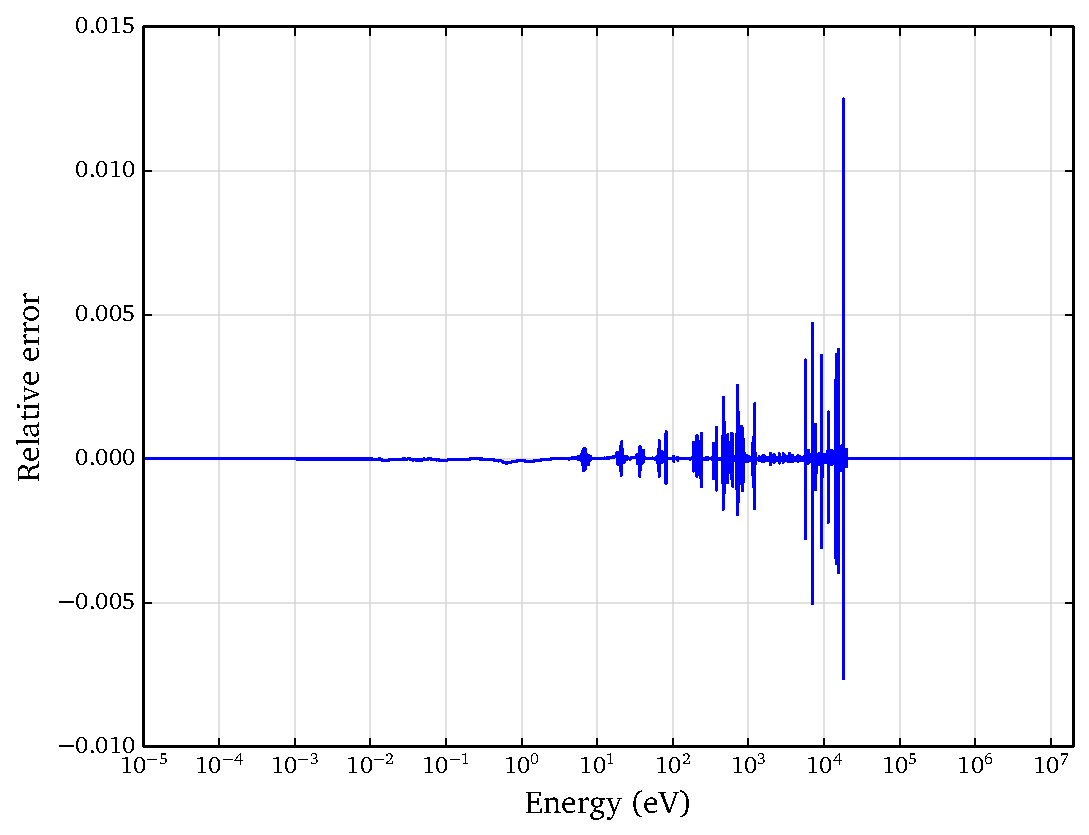
\includegraphics[width=4in]{plots/griderror.pdf}
  \caption{Relative error in the broadened $^{238}$U fission cross section
    produced using a 16 point Gauss-Hermite quadrature as a function of incoming
    neutron energy.}
  \label{fig:griderror}
\end{figure}

Rather than looking only at the maximum relative error, we chose to introduce
another metric to characterize the accuracy. Ultimately, errors in reaction
cross sections will manifest themselves as errors in observed reaction rates in
a simulation. Thus, the metric we use is the expected difference in
energy-integrated reaction rates given a flux spectrum:
\begin{equation}
  \label{eq:rr-metric}
  \frac{\int_0^{\infty} dE \; \left ( \sigma_{GH}(E) - \sigma(E) \right )
    \phi(E)}{\int_0^{\infty} dE \; \sigma(E) \phi(E)}
\end{equation}
where $\sigma_{GH}(E)$ is the cross section broadened using the Gauss-Hermite
quadrature and $\sigma(E)$ is the cross section broadened using the exact
integration method.  The choice of the flux spectrum will influence what errors
are most important. For the present work, a flux spectrum characteristic of a
typical pressurized water reactor (PWR) is used. \autoref{fig:spectrum} shows
the flux spectrum from the BEAVRS benchmark \citep{mc-horelik-2013}, which was
used for calculating \autoref{eq:rr-metric}, as calculated by OpenMC
\citep{ane-romano-2013}.
\begin{figure}[htbp]
  \centering
  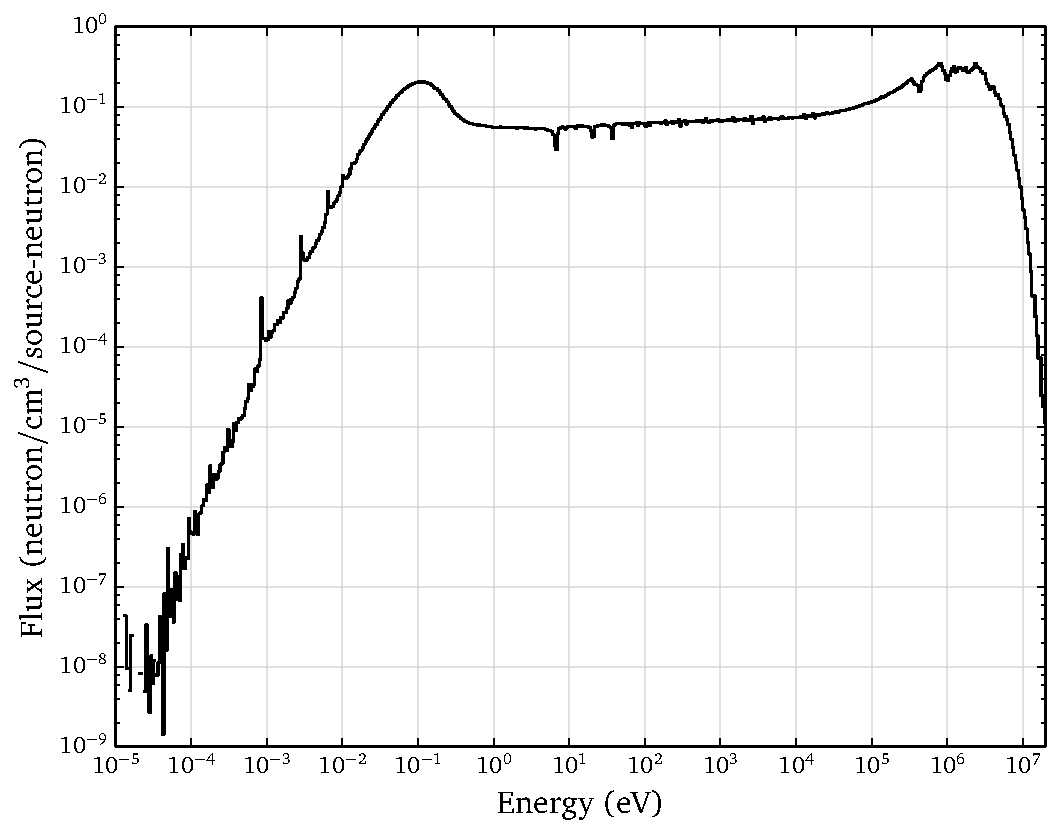
\includegraphics[width=4in]{plots/spectrum.pdf}
  \caption{Neutron flux spectrum in the BEAVRS benchmark model as calculated by
    OpenMC.}
  \label{fig:spectrum}
\end{figure}

With the metric in \autoref{eq:rr-metric}, we can now calculate both the maximum
relative error in each broadened cross section as well as its expected effect on
a reaction rate in a PWR spectrum. \autoref{fig:error-U238-total} shows the
maximum relative error over the full energy grid (solid lines) and the relative
difference in reaction rates (dashed lines) for the $^{238}$U total cross
section at three temperatures and as a function of the Gauss-Hermite quadrature
order. The maximum relative error in the cross section gradually decreases with
increasing quadrature order until it levels out at about $10^{-3}$ for
quadrature orders above 15. Similar behavior is observed for the expected error
in reaction rates, except that it is considerably lower than the maximum
relative error and settles out at $10^{-5}$. As expected, larger temperature
differences for broadening result in worse errors for lower quadrature orders,
but all cases asymptote to the same value.
\begin{figure}[H]
  \centering
  \includegraphics[width=4in]{plots/error_U238_n,tot.pdf}
  \caption{Error in the broadened $^{238}$U total cross section produced using a
    Gauss-Hermite quadrature as a function of the quadrature order. The solid
    lines represent the maximum absolute error across all grid points. The
    dashed lines represent the relative difference in the energy-integrated
    reaction rate using the flux spectrum from BEAVRS.}
  \label{fig:error-U238-total}
\end{figure}

The error plot for each nuclide and broadenable reaction looks qualitatively
similar to \autoref{fig:error-U238-total}, reaching a minimum error at
quadrature order between 15 and 20. This is not surprising considering that the
Gauss-Hermite quadratures with many points have abscissas that extend between
the range of integration normally considered for Doppler broadening ($-4 \le z <
4$). \autoref{fig:quadrature} shows the largest root of the Hermite polynomial
as a function of its order. It is important to note that the exact integration
method results which were used for comparison were calculated with an extended
range of integration, $-8 \le z < 8$.
\begin{figure}[H]
  \centering
  \includegraphics[width=4in]{plots/quadrature.pdf}
  \caption{Largest root of Hermite polynomial as a function of its order.}
  \label{fig:quadrature}
\end{figure}

\autoref{fig:error-U235-fission} and \autoref{fig:error-FE56-total} give two
more examples of relative errors for the $^{235}$U fission cross section and the
$^{56}$Fe total cross section, respectively. Interestingly, for the $^{56}$Fe
total cross section, the relative error in reaction rates has already reached
its minimum with a five point quadrature even though the maximum relative error
continues to decrease with increasing quadrature order.
\begin{figure}[H]
  \centering
  \includegraphics[width=4in]{plots/error_U235_n,totf.pdf}
  \caption{Error in the broadened $^{235}$U fission cross section produced using a
    Gauss-Hermite quadrature as a function of the quadrature order.}
  \label{fig:error-U235-fission}
\end{figure}
\begin{figure}[H]
  \centering
  \includegraphics[width=4in]{plots/error_FE56_n,tot.pdf}
  \caption{Error in the broadened $^{56}$Fe total cross section produced using a
    Gauss-Hermite quadrature as a function of the quadrature order.}
  \label{fig:error-FE56-total}
\end{figure}

One final observation is that the maximum relative error and the relative error
in reaction rates seem to be lower for even quadrature orders when compared to
odd quadrature orders.

\subsection{On-the-fly Doppler Broadening}

Given the excellent performance and accuracy of the Gauss-Hermite quadrature
method, it begs the question of whether it could be used effectively as an
on-the-fly method for Doppler broadening in a Monte Carlo code. In fact,
\citet{nd-dean-2010} had used the Gauss-Hermite method for on-the-fly broadening
in the MONK Monte Carlo code but said that it led to a factor of 10 increase in
run time.

A Doppler broadening algorithm using a Gauss-Hermite quadrature was implemented
in a developmental version of the OpenMC Monte Carlo code. In OpenMC, each time
the energy of a particle changes, the total, elastic, absorption, and fission
cross sections are calculated for each nuclide in the material that the particle
is in. However, not all reactions need to be broadened; it was assumed that only
non-threshold reactions need to be Doppler broadened. As a result, the
non-broadenable reactions were summed at the beginning of the simulation for
easy retrieval during cross section calculations. Note that several categories
of non-broadenable reactions were required in order to calculate the broadened
fission, absorption, and total cross sections.

The broadenable reactions were combined into a two dimensional array of size
$(N,M)$ where $N$ is the number of points on the energy grid and $M$ is the
number of broadenable reactions. This enables all reactions to be broadened at
once rather than having to broaden each one individually. Since no information
on the upper energy of the resolved resonance range (usually used as the cutoff
energy above which broadening is ignored) is contained in the ACE cross section
libraries, it was assumed that broadening should not be performed above
\SI{1}{\mega\electronvolt}.

To test the on-the-fly Doppler broadening implementation, a model of the BEAVRS
reactor benchmark was simulated. The cross sections used were generated by NJOY
at \SI{600}{\kelvin} and broadened to \SI{900}{\kelvin} during the
simulation. Since the run time is strongly dependent on the number of nuclides
in fuel, a series of runs was performed starting with 5 nuclides in fuel and
increasing the number up to 390 (the number of nuclides available in the cross
section library being used). \autoref{fig:otf} shows the fractional increase in
run time for this problem as a function of the number of nuclides in fuel. In
both the regular run using no Doppler broadening and the one for which Doppler
broadening was turned on, the run time increases greatly with an increasing
number of nuclides. The net effect in this case is that the overhead of the
Doppler broadening treatment tends to decrease with an increasing number of
nuclides but is considerably high for all values. The initial rise in the
fractional increase may be related to the fact that the nuclides being added in
the fuel first were light nuclides.
\begin{figure}[H]
  \centering
  \includegraphics[width=4in]{plots/otf.pdf}
  \caption{Fractional increase in run time due to on-the-fly Doppler broadening
    in the BEAVRS benchmark model as a function of the number of nuclides in
    fuel regions.}
  \label{fig:otf}
\end{figure}

The on-the-fly Doppler broadening was also tested for the Monte Carlo
performance benchmark \citep{mc-hoogenboom-2011} where it resulted in a factor
of nine increase in run time. This is more in line with the results quoted by
\citet{nd-dean-2010}, although no mention was made of what problem they had
simulated. With about an order of magnitude increase in run time for both the
BEAVRS and Monte Carlo performance benchmarks, the overhead is likely to be
unacceptably high for all but the simplest of problems.

%%%%%%%%%%%%%%%%%%%%%%%%%%%%%%%%%%%%%%%%%%%%%%%%%%%%%%%%%%%%%%%%%%%%%%%%%%%%%%%%
\section{Conclusions}

The present work helps to elucidate differences in speed and accuracy between a
number of methods used for Doppler broadening pointwise tabulated cross
sections. These methods are commonly used in cross section processing codes; as
evidenced by a number of recent works in the literature, there is generally a
desire to improve the performance of these processing codes.

Using a Gauss-Legendre quadrature to perform integration over smooth
subintervals when broadening was found to reduce broadening time by 48\% on a
small test suite when compared to the exact integration method using an
implementation of the $\erfc$ function from NJOY. However, just changing the
$\erfc$ implementation to the Fortran 2008 intrinsic resulted in a 35\% decrease
in run time as well.

Using a Gauss-Hermite quadrature offers a much greater improvement in
performance due to the fact that the number of cross section lookups required to
broaden a single point is limited by the order of the quadrature rather than the
density of points on the energy grid. This has the greatest effect for nuclides
with many resonances. The observed run time for the test suite using the
Gauss-Hermite quadrature varied between 2 and 3 seconds depending on the order
of the quadrature, over a factor of 10 less than the time required for the exact
integration method using NJOY's $\erfc$ function.

A study of the maximum relative error in broadened cross sections and the
expected relative error in energy-integrated reactions rates in a PWR spectrum
as a function of the quadrature order showed that orders of 15 or above reach an
asymptotic error level. Maximum relative errors generally were reduced to
approximately 0.1\%, whereas relative errors in energy-integrated reactions
rates were generally $10^{-5}$ or less. In a global sense, this implies that,
for an eigenvalue calculation, the use of these cross sections is not expected
to result in errors in reactivity of much more than a few pcm.

An implementation of the Gauss-Hermite method in OpenMC for on-the-fly Doppler
broadening resulted in a run time overhead comparable to that observed by
\citet{nd-dean-2010}, generally at least an order of magnitude compared to a
simulation without Doppler broadening. Given that a number of optimization
techniques were already used in the OpenMC implementation, e.g., coalescing all
broadenable reactions into one two-dimensional array, it is unlikely that
further improvements could be made in the serial code. However, there may be
opportunities for improvements in an on-the-fly implementation by taking
advantage of specialized single instruction, multiple data (SIMD) hardware such
as GPUs or co-processors. Either way, the results underscore the need for
advanced methods for on-the-fly temperature treatment in Monte Carlo codes.

%%%%%%%%%%%%%%%%%%%%%%%%%%%%%%%%%%%%%%%%%%%%%%%%%%%%%%%%%%%%%%%%%%%%%%%%%%%%%%%%
\section*{References}

\bibliographystyle{elsarticle-harv}
\bibliography{references}

\end{document}
